%% ID: momentum
%% VIDEO: c_of_e
%% QUESTIONS: head_on_collision, what_goes_up
%% LEVEL: 2
%% TOPIC: physics/mechanics/dynamics
%% TYPE: concept
%% LINKTITLE: Momentum

% This is the template that sets out all of the Problems and produces the Exercise/Solution labels and numbering
% There are two classes of Exercise: "problem" which has a Question and Solution, and "hint" which has a Question, Hint and Solution

% This is the template that sets out all of the Problems and produces the Exercise/Solution labels and numbering
% There are two classes of Exercise: "problem" which has a Question and Solution, and "hint" which has a Question, Hint and Solution

% These are the packages to use in all documents, and the paper size to use:
\documentclass[a4paper,11pt]{article}
\usepackage[usenames,dvipsnames]{xcolor}
\usepackage[margin=1.5cm]{geometry}
\usepackage{amsmath}
\usepackage{amssymb}
\usepackage{color}
\usepackage{graphicx}
\usepackage{graphics}
\usepackage[margin=1.5cm]{geometry}
\usepackage{fancyhdr}
\usepackage{float}
\usepackage{lscape}
\usepackage[font={small},labelfont=bf]{caption}
\usepackage{ifthen}
\usepackage{enumitem}
\usepackage{subcaption}		%Allows grouped figures. The percentage sign after the first \end{subfigure} puts them side by side, omitting it puts one above the other.
\usepackage{graphicx,xcolor} 	%Allows the use of colour in the files
\usepackage{centernot} 		%Puts the / in a not equal to sign in the centre, use as \cnot{...}
\usepackage{comment} 		%Allows \begin{comment} .... \end{comment} to comment out bulk text.
\usepackage{etoolbox}		%Allows the boolean flags and the \toggletrue and \togglefalse commands
\usepackage{cancel}		%Allows the crossing out of terms in maths mode to show they cancel out
\usepackage{wrapfig}

%Packages for font choices
\usepackage{palatino}
\usepackage{mathpazo}


%Then where to find the graphics:
%WARNING -  relative to the TeX file being compiled - NOT this template!
		\graphicspath{{../Diagrams/}{Diagrams/}{./}} %This allows diagrams: {{As a sister folder to Latex}{A subdirectory of LaTeX}{Or just in LaTeX itself}}

% WARNING -  If you want the diagrams to be a sister folder to the LaTeX folder - pdflatex.exe sometimes needs an extra argument to cope with the "../" part; usually it can only cope with subdirectories as opposed to parent ones. If it refuses to compile and says it cannot find the diagrams, either add "--shell-escape" to the start of the arguments of pdflatex, OR move the diagrams to a subdirectory of the one containing the TeX files.
%In TeXworks, to add the extra argument, go to Edit -> Preferences -> Typesetting -> Processing Tools. Click on "pdfLaTeX" -> Edit -> "+" button, then type "--shell-escape" (without quotes) and press the up arrow twice so that it becomes top of the list.


%Then any custom commands written, along with shortcuts and variables:
% This document contains any custom commands, shortcuts and variables needed for the files to compile. It is called by "Problem_Template.tex" and so needs to be in the same directory.

%Defines vectors universally, for ease of editing and consistency.
\newcommand{\vtr}[1] {\mathit{\underline{\boldsymbol{#1}}}}

%Draws a big red box containing the text as in \ALERT{<TEXT HERE>}. For labelling draft copies with important notes.
\def\ALERT#1{\begin{center}\colorbox{red}{\hbox{\textcolor{black}{\textbf{#1}}}}\end{center}}

%Roman-style subscript; removes math-mode font.
\def\s#1{_\textrm{#1} }

%The operators in integrals and derivatives.
\def\d{\operatorname{d}\!}

%The Euler e should be in Roman font.
\def\e{\textrm{e}}

%The Rutherford title, to save typing and for consistency:
\def\Rutherford{Rutherford School Physics}
\def\Concepttitle#1{\noindent\textsc{\Rutherford\vspace{0.4cm}\\ \LARGE Physical Concept: \textbf{#1}}}
\def\Problemtitle#1{\noindent\textsc{\Rutherford\vspace{0.4cm}\\ \LARGE Website Problems: \textbf{#1}}}
\def\AddProblemtitle#1{\noindent\textsc{\Large \Rutherford ~ --- ~ Additional Problems\vspace{0.4cm}\\ \LARGE \textbf{#1}}}
%\def\AddProblemtitle#1{\noindent\textsc{\Rutherford\vspace{0.4cm}\\ \LARGE Additional Problems: \textbf{#1}}}

%define quick question to be used in eg concept sheet.
%\def\qq#2{#1}{\color{red}[#2]\color{black}}
\newcommand{\qq}[2]{\nl Quick Question:\hspace{1 mm} #1\color{red}\hspace{2 mm} Answer:\color{black}\hspace{1 mm}  #2}
\newcommand{\stress}[1]{\emph{#1}}

%%%%%%%%%%%   some definitions used in latexing the CQMP:
% fractions that are of right size in set equations
\def\half{{\textstyle \frac{1}{2}}}
\def\quarter{{\textstyle \frac{1}{4}}}
\def\third{{\textstyle \frac{1}{3}}}
\def\eighth{{\textstyle \frac{1}{8}}}

% obtain a new line
\def\nl{\hfil\break}
\def\nll{\\ \\ \noindent}



%creates numbered lists with a), then i.
\renewcommand{\theenumi}{\alph{enumi}}% first level are latin characters
\renewcommand{\labelenumi}{\theenumi)} %tells it to put a bracket after the character.
\renewcommand{\theenumii}{\roman{enumii}}%second level are little roman characters
\renewcommand{\labelenumii}{\theenumii.} %tells it to put a dot after the character
 % In a file called "Definitions.tex" in the same directory as this file.

%Define some boolean switches:
\newtoggle{solutions_only}	%Print only the solutions
\newtoggle{no_solutions}		%Don't print any solutions  (overridden by solutions_only)
\newtoggle{solutions_at_end}	%Print the solutions at end (overridden by solutions_only and no_solutions)
\newtoggle{no_credits}		%Don't print the credit arguments

%Use this to write a list of things needed to know for a section. It automatically won't print when "solutions_only" is on.
%Its only argument should be a list of things needed to know in "\item [....]" form
\newenvironment{knowledge}[1]{
\iftoggle{solutions_only}{}{It is assumed that students will be familiar with the following concepts:
\begin{itemize} #1 \end{itemize}
\vspace{0.5cm}}
}

%Allows the headings to be managed when not printing problems ect.
\newenvironment{Qsection}[1]{
%\iftoggle{solutions_only}{}{\section{#1}} %Don't output headings in the solutions(?)
\iftoggle{solutions_at_end}{\AtEndDocument{\section{#1}}}{}
\section{#1}
}

\newenvironment{Qsubsection}[1]{
%\iftoggle{solutions_only}{}{\subsection{#1}} %Don't output headings in the solutions(?)
\iftoggle{solutions_at_end}{\AtEndDocument{\subsection{#1}}}{}
\subsection{#1}
}

%Set the values of the boolean switches: Yes - "toggletrue", No - "togglefalse".
\togglefalse{solutions_only}	%	ONLY		Output only solutions? 
\togglefalse{no_solutions}		%	NONE		Don't output solutions at all? 
\togglefalse{solutions_at_end}	%	END		Output solutions at the end?
\togglefalse{no_credits}		%			Don't output the credit field
%All 8 cases have been tested; ONLY takes precedence, then NONE and finally END is lowest.


%##############################################################################################################
%											Then the bulk of the layout options:
%##############################################################################################################

\setlength{\topmargin}{-2cm}
%\setlength{\oddsidemargin}{0.5cm}
%\setlength{\evensidemargin}{0.5cm}


%##############################################################################################################


\newcounter{exercisenumber}%[chapter] %counter is set to zero when "chapter" appears
\def\theexercisenumber{\arabic{exercisenumber}}


\iftoggle{no_solutions}{}{ %Put a header at the end before the solutions, and reset the counter. Only if solutions are being printed AND at the end.
	\iftoggle{solutions_only}{}{
		\iftoggle{solutions_at_end}
			{\AtEndDocument{\newpage \part*{Solutions:} \setcounter{exercisenumber}{0} \setcounter{section}{0}}}{}
	}
}


%%%%%%%%%%%%%%%%%%%%%%%%%%%%%%%%%%%%%%%%%%%%%%%%%%%%%%%%%%%%%%%%%%%%%%%%%%%%%%%%%
%Creates \begin{problem}[label]{exercise_text}{source_text}{solution_text}\end{problem} command - the label argument is optional
%If put in, remember to put in [] brackets.  A label called label.ex will be generated.
\newenvironment{problem}[4][noref]{
 \refstepcounter{exercisenumber} %\refstepcounter allows you to reference to the exercise number
%
\iftoggle{solutions_only}{\hfil\break \textit{Solution}~\theexercisenumber:  #4}{ %If only solutions, just output solution.
	\noindent{\textit{Exercise}~\theexercisenumber:}
	\ifthenelse{\equal{#1}{noref}}{}{\label{#1.ex}} #2 %\vspace{0.3cm}
	\iftoggle{no_credits}{}{
			%\hfil\break {\small #3} \vspace{0.3cm} %This is the old line, replaced with the one below, without the ifthenelse statement; in case something goes wrong.
			\ifthenelse{\equal{#3}{}}{}{ {\tiny [#3]} \vspace{0.3cm}} %If the credit field is blank; don't bother printing it or the space for it.
	} %reference argument
%
	\iftoggle{no_solutions}{}{ %If the solutions aren't to be printed, do nothing.
		\iftoggle{solutions_at_end}
			{\AtEndDocument{\stepcounter{exercisenumber}\hfil\break \textit{Solution}~\theexercisenumber:  #4 \vspace{0.5cm}}} %If at the end: do this.
			{\hfil\break \textit{Solution}~\theexercisenumber:  #4} 	%Else leave in line as in TeX file.
	}
}

\vspace{0.2cm}}

%%%%%%%%%%%%%%%%%%%%%%%%%%%%%%%%%%%%%%%%%%%%%%%%%%%%%%%%%%%%%%%%%%%%%%%%%%%%%%%%%
%Creates \begin{hint}[label]{exercise_text}{hint_text}{source_text}{solution_text}\end{hint} command - the label argument is optional
%If put in, remember to put in [] brackets.  A label called label.ex will be generated.
\newenvironment{hint}[5][noref]{
 \refstepcounter{exercisenumber}
%
\iftoggle{solutions_only}{\hfil\break \textit{Solution}~\theexercisenumber:  #5}{  %If only solutions, just output solution.
	\noindent{\textit{Exercise}~\theexercisenumber:}
	\ifthenelse{\equal{#1}{noref}}{}{\label{#1.ex}} #2 \vspace{0.1cm}
	 \hfil\break  \textit{Hint:}  #3{} %\vspace{0.3cm}
	\iftoggle{no_credits}{}{
			\ifthenelse{\equal{#4}{}}{}{\\ \hfil {\tiny #4} \vspace{0.3cm}} %This is the old line, replaced with the one below, without the ifthenelse statement; in case something goes wrong.
			%\ifthenelse{\equal{#4}{}}{}{{\tiny [#4]} \vspace{0.3cm}} %If the credit field is blank; don't bother printing it or the space for it.
	} %reference argument
%
	\iftoggle{no_solutions}{}{%If the solutions aren't to be printed, do nothing.
		\iftoggle{solutions_at_end}
			{\AtEndDocument{\stepcounter{exercisenumber}\hfil\break \textit{Solution}~\theexercisenumber:  #5 \vspace{0.5cm}}} %If at the end: do this.
			{\hfil\break \textit{Solution}~\theexercisenumber:  #5}%Else leave in line as in teX file.
	}
}
\vspace{0.2cm}}

%%%%%%%%%%%%%%%%%%%%%%%%%%%%%%%%%%%%%%%%%%%%%%%%%%%%%%%%%%%%%%%%%%%%%%%%%%%%%%%%%


 %%%%%%%
\newenvironment{additional}[2][noref]{
 \refstepcounter{exercisenumber}
% \vspace{.2cm}
\nl
\noindent{\textit{Exercise}~\theexercisenumber:}
\ifthenelse{\equal{#1}{noref}}{}{\label{#1.ex}} #2 }{%\vspace{5.1cm}
 }
%










% to mark as a draft.  Comment both these lines out when complete.  The page number will return to the footer.
%\pagestyle{myheadings}
%\markright{\textcolor{red}{\textbf{DRAFT: \today}}}

\begin{document}
\addtolength{\topmargin}{-0.7 cm}
\setlength{\columnsep}{22pt}
\Concepttitle{Momentum and its conservation;\nl collisions --- Part 1.}
\nll
We briefly sketch definitions of momentum.  Understanding momentum further involves revising Newton's Laws and ideas about impulse, which are available at greater length at the concepts pages for Newton's Laws and for Impulse.  Collisions are a good area for illustration.  Part 2 for this concept addresses more powerful techniques for dealing with collisions, for instance as they arise in particle physics.

\section{Definition of momentum}
Momentum is mass $m$ times velocity $\vtr{v}$ for a particle: $\boxed{\vtr{p} = m \vtr{v}}$.\nll
It is a vector with units kg.m/sec.  Momentum can be carried by other entities, such as waves, but we just sketch mechanical momentum.

\section{Conservation of momentum}
The momentum is conserved in the absence of forces external to the system.  \\
This concept is one of the most important in physics and follows from Newton's laws.  Newton's second law (N2L, ``force = mass times acceleration") can be written:
\begin{equation*} \vtr{f} = m \vtr{a} = m \d\vtr{v}/\d t = \d\vtr{p}/\d t .
\end{equation*}
N1L says that in the absence of forces, particles continue moving without further change of velocity.  Setting $\vtr{f}= 0$ in the above shows that then $\vtr{v}$ is unchanging, as is momentum $\vtr{p}$, that is momentum is conserved.\nll
Consider a system consisting of two particles colliding head on, figure~\ref{fig:collision}. The box indicates the system is ``closed" --- there are forces within it (when the particles collide), but not on it from outside.
\nll
Momentum is always conserved, but energy can be converted to other forms (e.g. to heat) so collisions may or may not be elastic (that is conserving mechanical energy).  So one has:
\begin{equation*} \vtr{p}_1 +  \vtr{p}_2 = \vtr{p}_1'  + \vtr{p}_2'
\end{equation*}
where the prime $'$ indicates after the collision.
\begin{figure}[h!]% this one for two figures side by side
\centering
\begin{minipage}{.45\textwidth}
  \centering
  \includegraphics[width=0.7\linewidth]{figures/collision.eps}
  \caption{The collision of two particles isolated from the rest of the world.}
  \label{fig:collision}
\end{minipage}\hfil
\begin{minipage}{.45\textwidth}
  \centering
  \includegraphics[width=0.45\linewidth]{figures/inelastic.eps}
  \caption{The inelastic collision of two particles that stick together after colliding.}
  \label{fig:inelastic}
\end{minipage}
\end{figure}
\vspace{-0.5cm}
\subsection*{Levels 1--4.  Questions:}
\begin{itemize}
\item[1.]  Figure~\ref{fig:inelastic} shows two particles colliding and then sticking together.\\
If $m_1 = 1 \textrm{kg}$, $m_2 = 2\textrm{kg}$, $v_1 = 3 \textrm{m s}^{-1}$ and
$v_2 = 1\textrm{m s}^{-1}$, then the momentum is $1 \times 3 + 2 \times 1  = 5 \textrm{kg m s}^{-1}$.
It remains this value and hence after the collision one has $5 \textrm{kg m s}^{-1} = 3 \textrm{kg} \times v' \; \textrm{m s}^{-1}$.  Thus $ v' = 5/3 \; \textrm{m s}^{-1}$.
\nl
Calculate how much energy has been lost in the collision by calculating the total kinetic energy before and after.\\
Describe the collision (with sticking) in the case $m_1 = m_2 = 1\textrm{kg}$.\\

\item[2.]  Consider two particles of equal mass, $m_1 = m_2 = m$ where $v_1 = v$ simply, and the other particle is initially at rest, $v_2=0$.  They collide elastically; see figure~\ref{fig:elastic}.  What are the final speeds $v_1'$ and $v_2'$?

\end{itemize}
\begin{figure}[h!]% this one for two figures side by side
\hspace{1.0cm}
\begin{minipage}{.45\textwidth}
  \centering
  \includegraphics[width=.8\linewidth]{figures/elastic.eps}
  \caption{An elastic collision of two equal particles, one being initially at rest.}
  \label{fig:elastic}
\end{minipage}\hspace{0.2cm}
\begin{minipage}{.45\textwidth}
  \centering
  \includegraphics[width=.45\linewidth]{figures/wall.eps}
  \caption{A particle colliding with a wall.  In the intermediate state it is instantaneously at rest and deformed.}
  \label{fig:wall}
\end{minipage}
\end{figure}

\begin{itemize}
\item[] Conserving momentum gives: $m v = m (v_1' + v_2')$ hence $v = v_1' + v_2'$.\\
Conserving energy gives: $\half m v^2 = \half m (v_1'^2 + v_2'^2)$.  Hence
$v^2 = v_1'^2 + v_2'^2$.
\nl
Put $v_1'  = v - v_2'$ from above into this energy relation:
\begin{equation*} v^2 = (v - v_2')^2 + v_2'^2  = v^2 - 2 v v_1' +v_1'^2 + v_1'^2\nl
\rightarrow 2 v v_2' = 2 v_2'^2  \rightarrow v_2' = v .
\end{equation*}
Put this value of $v_2'$ into the momentum relation and find that $v_1' = 0$.\nl

The first particle stops and the second continues with the velocity (and momentum) of the first --- like in Newton's cradle.
\item[3.]  A particle bouncing off a wall; figure~\ref{fig:wall}.\\
The incident particle has a force from the wall acting on it during the collision.  Momentum of the particle is not conserved. But \textit{the total momentum} of the particle plus the wall \textit{is conserved}.\\
  What is the change of momentum if the collision is elastic? (Remember momentum and its changes are vectors -- your answer requires a magnitude and a direction.)\\
 What is the momentum change if the collision is completely inelastic?
\end{itemize}

\section{Impulse}
Impulse is the change of momentum.  It is force times time, for a constant force acting.  The term is generally (but not always) used when momentum is transferred over a short time (e.g. during a collision).  It is described fully in the impulse concepts sheet.

\end{document}
